\chapter{\uppercase{Human-Inspired Control}} \label{ch:hic}

The human-inspired control framework is based on the idea of designing robotic
behaviors based on kinematic analysis of human motion.
%
Originally applied to a four-domain hybrid model of a robot with feet and knees
\cite{Sinnet2011b} in two dimensions, the method was later found to apply to a
wide range of models including the compass-gait biped \cite{Sinnet2011a} and
hybrid human--robot simulations of a human with a transfemoral prosthesis
\cite{Sinnet2011}.
%
By combining human-inspired control with functional Routhian reduction,
three-dimensional walking was also achieved \cite{Sinnet2012a, Sinnet2012}.
%
This chapter discusses the basics of human-inspired control method.

\section{Domain Breakdown from Human Data} \label{sec:domainbreakdown}

This section shows how to determine the domain breakdown for human walking.
%
The procedure provided is a data-driven approach based on a prior experiment
involving human test subjects documented in \cite{Ames2011a}.
%
First, a discussion is given on the human experiment and how the data were
handled. 
%
Then a method is presented for determining the domain breakdown by finding the
times when the constraint for a given contact point is enforced through a method
that fits the ``simplest'' function to the motion of the contact point when the
constraint is not enforced (or, in other words, when the contact point is not in
contact with the ground);
%
the time intervals during a step when the constraints are enforced are simply
the times when this function is not being followed.
%
The end result of this procedure is a temporal ordering of events which creates
a discrete structure termed the domain breakdown.

Application of the presented method to each of the tests subjects results in an
identical domain breakdown for each subject, purporting that there is indeed a
{\em universal} domain breakdown for healthy human walking.
%
This result is a significant step toward understanding human walking.
%
Accordingly, this universal domain breakdown will be considered when
constructing the hybrid model of the biped of interest.
%
This domain breakdown has been used to formulate a metric on the human-like
nature of robotic walking gaits \cite{Ames2011, Vasudevan2013}.

\begin{figure}[t!]
  \centering
  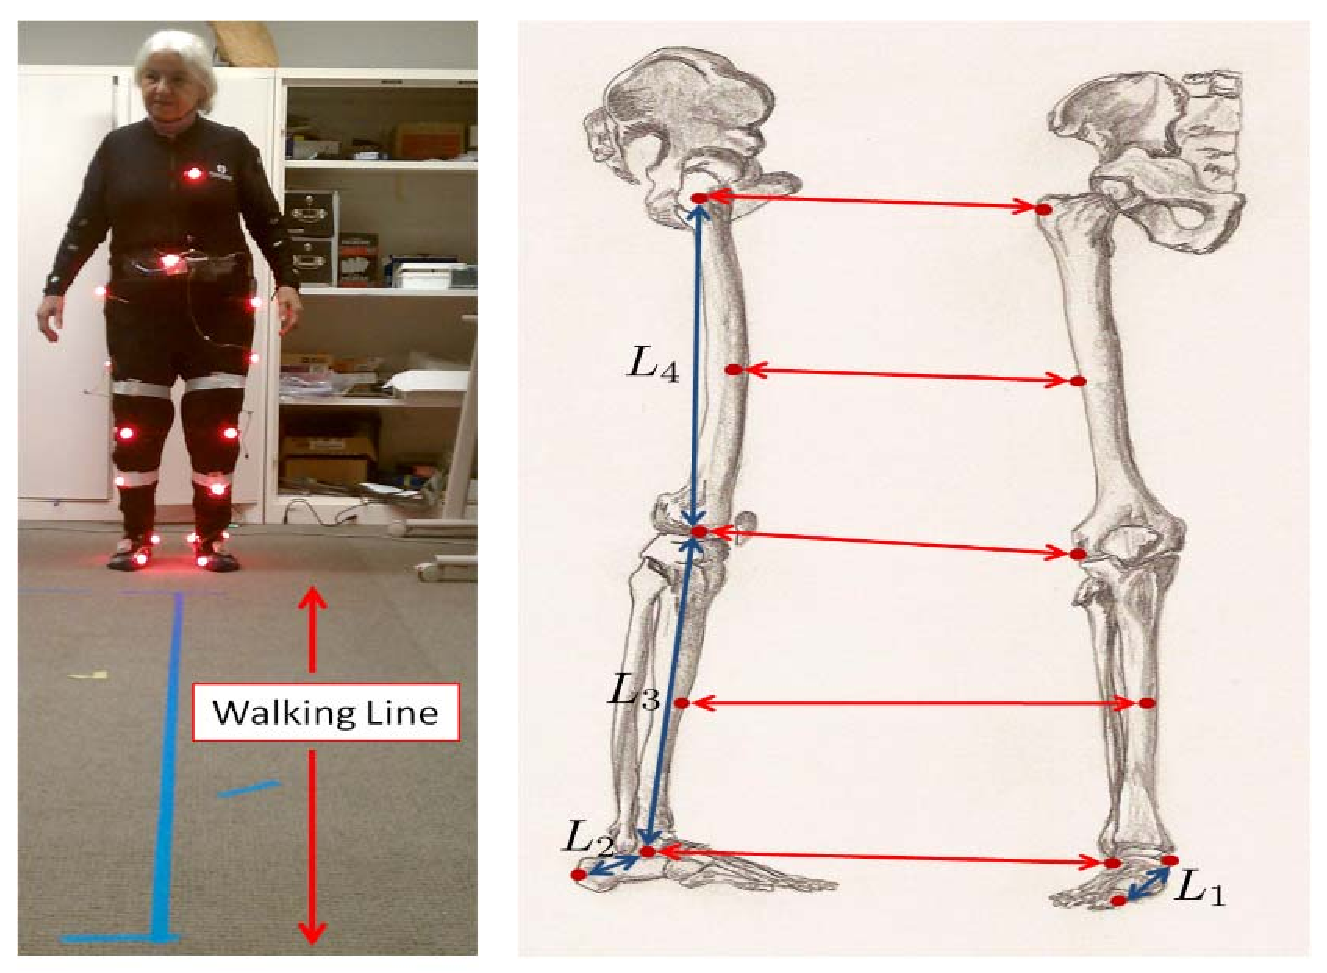
\includegraphics[width=0.7\textwidth]{LabeledDiagram}
  \caption[Illustrations of the experimental setup and sensor
  placement.]{Illustrations of the experimental setup (left) and sensor
    placement (right).
    %
    Each subject in the experiment was required to wear a suit where the LED
    sensors are fastened in place.
    %
    The sensors were placed at the joints as illustrated with the red dots on
    the right lateral and anterior aspects of the right leg.
    %
    Sensors were placed identically on the left leg.
    %
    The same sensors drawn from different views are connected with red arrows.
    %
    The blue arrows illustrate the leg segment lengths of interest,
    i.e. $L_{1}$, $L_{2}$, $L_{3}$, $L_{4}$.
    %
    The diversity of the subjects with respect to these lengths can be seen in
    \tabref{tab:measurements}.}
  \label{fig:Sensors}
\end{figure}

\begin{table}[t!]
  % \HRule
  % \vspace{2mm}

  \centering
  \caption[Measurements describing each of the subjects.]{Measurements
    describing each of the subjects.
    %
    The subject number is in the left column and the $L_1,L_2,L_3,L_4$
    measurements correspond to the lengths described in \figref{fig:Sensors}.
    %
    The anthropometric measurements in column $4$ are in kilograms and the
    measurements in columns $5$--$9$ are in centimeters.}
  \begin{tabular}{|c|c|c|c|c|c|c|c|c|}
    \hline
    & \!Sex\! & \!Age\! &  \!Weight\! & \!Height\! & $L_1$ & $L_2$ & $L_3$ &
    $L_4$ \\ \hline
    1 & M & 30 & 90.7& 184& 14.5& 8.5& 43.0& 44.0 \\ \hline
    2 & F & 19 & 53.5& 164& 15.0& 8.0& 41.0& 44.0\\ \hline
    3 & M & 17 & 83.9& 189& 16.5& 8.0& 45.5& 55.5 \\ \hline
    4 & M & 22 & 90.7& 170& 14.5& 9.0& 43.0& 39.0\\ \hline
    5 & M & 30 & 68.9& 170& 15.0& 8.0& 43.0& 43.0\\ \hline
    6 & M & 29 & 59.8& 161& 14.0& 8.5& 37.0& 40.0\\ \hline
    7 & M & 26 & 58.9& 164& 14.0& 9.0& 39.0& 41.0\\ \hline
    8 & F & 77 & 63.5& 163& 14.0& 8.0& 40.0& 42.0\\ \hline
    9 & F & 23 & 47.6& 165& 15.0& 8.0& 45.0& 43.0\\ \hline
  \end{tabular}
  \label{tab:measurements}
\end{table}


\begin{figure}[t!]
  \centering
  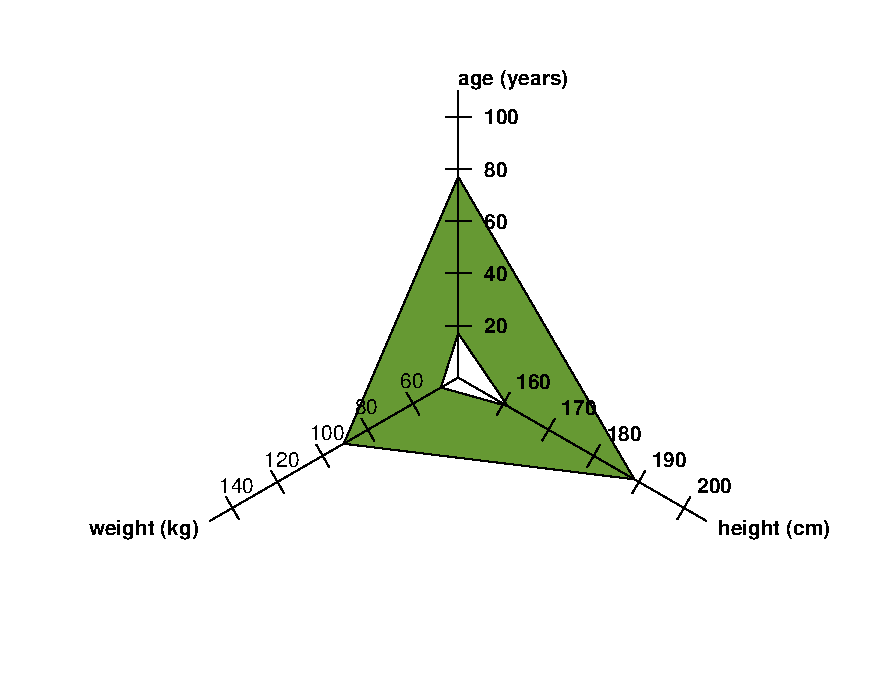
\includegraphics[width=0.7\textwidth]{subject_range_graph}
  \caption{The ranges of age, height, and mass of the test subjects.}
  \label{fig:subject-ranges}
\end{figure}

\subsection{Walking Experiment}

The data used in this work are taken from an experiment described in
\cite{Ames2011a}.
%
A summary of the collection procedure is provided for reference:
%
data were collected on nine subjects using the Phase Space System%
%
\footnote{\url{http://www.phasespace.com/}}\xspace
%
which computes the 3D position of $19$ LED sensors at $480$ frames per second
using $12$ cameras.
%
The cameras were calibrated prior to the experiment and were placed to achieve a
one millimeter level of accuracy for a space of size five by five by five meters
cubed.
%
Eight LED sensors were placed on each leg at the joints and on the heel and toe
as shown in \figref{fig:Sensors}, one LED sensor was placed on the sternum, one
LED sensor was placed on the back behind the sternum, and one LED sensor was
placed on the umbilicus.

\begin{figure}[t!]
  \centering
  \subfloat[Heel height]{
    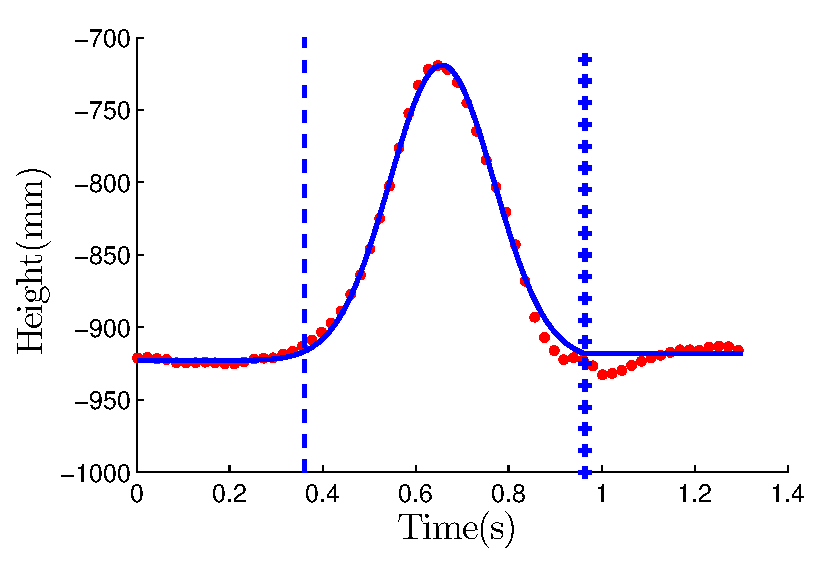
\includegraphics[width=0.48\columnwidth]{LeftHeel}
    \label{fig:heelheight}
  }
  \subfloat[Toe height]{
    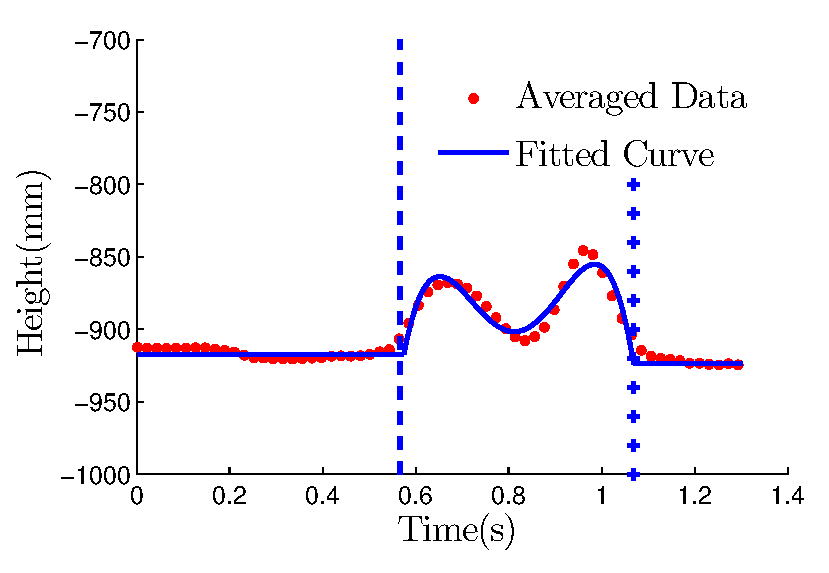
\includegraphics[width=0.48\columnwidth]{LeftToe}
    \label{fig:toeheight}
  }
  \caption[The data for the heights of the heel and toe.]{The data for the
    heights of the heel and toe.
    %
    Also shown are the fittings of a constant$\to$Gaussian$\to$constant for the
    heel and a constant$\to$fourth-order polynomial$\to$constant for the toe.
    %
    The vertical lines on the left and right indicate the lift and strike times,
    respectively.}
  \label{fig:heeltoefit}
\end{figure}

Each trial of the experiment required the subject to walk three meters along a
straight line drawn on the floor.
%
Each subject performed $12$ trials which constituted a single experiment.
%
Three female and six male subjects were tested with ages ranging between $17$
and $77$ years, heights ranging between $161$ and $189$ centimeters, and masses
ranging between $47.6$ and $90.7$ kilograms.
%
\tabref{tab:measurements} describes the measurements of each of the subjects and
a visual representation is given in \figref{fig:subject-ranges}.
%
The data for each individual were rotated so the walking occurs in the
$x$-direction and, for each subject, the $12$ walking trials were averaged
(after appropriately shifting the data in time) which resulted in a single
trajectory for each constraint for each subject for at least two steps (one step
per leg); the resulting data can be seen in \figref{fig:heeltoefit}.


\subsection{Function Fitting}

In order to determine the domain breakdowns for the subjects in the walking
experiment, it is necessary to determine the times when the human--ground
contact points change, i.e., the {\em event times}.
%
Rather than looking for when the contact point is constrained (through
thresholds), one can look for the ``simplest'' function that the contact point
follows when not enforced.
%
Then, for the domains in which the constraint {\em is not} enforced, use the
simple function; in the other domains, those in which the constraint {\em is}
enforced, fit a flat line to the constraint as it should be essentially
constant.
%
This is an optimization problem which can be stated as follows:
\begin{enumerate}
\item Select a simple function which is qualitatively similar to the trajectory
  of the constraint in the domains in which it is not enforced and choose an
  initial guess for the event times.
\item Create the fitted function as a piecewise combination of the chosen
  function fitted to the data in the domains in which the constraint {\em is
    not} enforced and a flat line fitted to the data in the domains in which
  the constraint {\em is} enforced.
\item Compute the cost function as the sum of squares of the difference between
  the data and value of the fitted trajectory at each datum for one full step
  (one step with each leg).
\item Minimize the cost function by choosing a new guess for the event times
  and then repeating steps 2--4.
\end{enumerate}

To formalize the idea of function fitting to determine event times, given a set
of contact points $\C$, let $s_{c}(t, a_{c})$ be the ``simplest'' function that
a given contact point $c \in \C$ follows when not in contact with the ground;
%
here $a_{c} \in R^{n_{c}}$ is a collection of parameters for the function
$s_{c}(t, a_{c})$ corresponding to contact point $c$.
%
Denote the indexed human data for contact point $c$ by $y_{c}[k]$, with
$\tau[k]$ the time corresponding to datum $y_{c}[k]$ for discrete index variable
$k \in \{1,\ldots,T\}$.
%
When the contact point is constrained, it is constant, and when it is
unconstrained, it follows $s_{c}(t, a_{c})$.
%
For each contact point $c \in \C$, consider the function:
%
\begin{align*}
  f_{c}(t, k_{c}^{\ell}, k_{c}^{s}, a_{c}) =  \left\{\begin{array}{l l}
      s_{c}(\tau[k_{c}^{\ell}], a_{c}), & \hspace{2mm} t \leq
      \tau[k_{c}^{\ell}],\\
      s_{c}(t, a_{c}), & \hspace{2mm} \tau[k_{c}^{\ell}] < t <
      \tau[k_{c}^{s}],\\
      s_{c}(\tau[k_{c}^{s}], a_{c}), & \hspace{2mm} \tau[k_{c}^{s}] \leq t,\\
  \end{array} \right.
\end{align*}
where $\tau[k_{c}^{\ell}], \tau[k_{c}^{s}] \in \{\tau[k]\}_{k = 1}^{T}$ are the
event times indicating when contact point $c$ becomes unconstrained (lift) and
constrained (strike), respectively.
%
It is assumed that $k_{c}^{\ell} < k_{c}^{s}$.
%
If this is not the case, then $f_{c}$ would consist of the ``simplest''
function, followed by a constant, followed by the ``simplest'' function.
%
After the construction of the $f_{c}$ functions in this chapter, the optimization
parameters are supressed---i.e., $f_{c}(t) = f_{c}(t, k_{c}^{\ell}, k_{c}^{s},
a_{c})$---but it is assumed they have been determined.
%
To calculate the event times as they best fit the data, one must solve the
following optimization problem
\begin{align*}
  \min_{k_{c}^{\ell}, k_{c}^{s} \in \{1, \ldots, T\}} \ \min_{a_{c} \in
    \R^{n_{c}}} \ \sum_{k = 1}^{T} \left( f_{c}(t, k_{c}^{\ell}, k_{c}^{s},
    a_{c}) - y_{c}(t) \right)^2
\end{align*}
for each $c \in \C$.
%
In the case of humans with flat feet, there are four constraints of interest:
%
one at the heel and one at the toe for both the left and right feet.
%
Since each constraint has a lift and strike time, there is a total of eight
domains in one whole step.
%
However, when referring to a step in robotics, researchers typically use stance
and non-stance legs;
%
without the distinction of left and right, the system is reduced to a
four-domain model.
%
Doing this allows one to exploit the symmetry inherent in bipedal walking to
simplfy controller design.

To illustrate this procedure, consider the averaged data for the heel and toe
shown in \figref{fig:heeltoefit}.
%
Looking at these data, the trajectory of the heel appears to follow a constant,
followed by a Gaussian, followed by a constant.
%
In a similar fashion, the averaged data for the toe appear to follow a constant,
followed by a fourth-order polynomial, followed by a constant.
%
With these observations in hand, fit the averaged heel and toe data to these
functions using the described procedure.
%
The results of the fitting procedure are shown in the topmost graph of
\figref{fig:heeltoefit};
%
the transition points $\tau[k_{c}^{\ell}]$ and $\tau[k_{c}^{s}]$ are indicated
by vertical lines.
%
The fits quite accurately represent the data given the simplicity of the
functions chosen;
%
to quantify this, the coefficients of correlatation are $0.9968$ for the heel
and $0.9699$ for the toe.


\subsection{Determining the Domain Breakdown}

Given the data for a contact point $c \in \C$, the lift and strike times are
determined for each contact point, $\tau[k_{c}^{\ell}]$ and $\tau[k_{c}^{s}]$
for $c \in \C =  \{c_{1},c_{2},c_{3},c_{4}\} = \{\clh, \clt, \crh, \crt\}$, over
the time interval of the averaged data, $\big[\tau[1], \tau[T]\big]$, using the
aforementioned techniques.
%
Since the data comprise at least two steps (one step with each leg), there are
multiple lift and strike times over the period of the data.
%
Denote by $\mathcal{J}_{c} \subset \big[\tau[1], \tau[T]\big]$ the period where
the constraints associated with a contact point are enforced, i.e., $t \in
\mathcal{J}_{c}$ if $f_{c}(t) = \mathrm{constant}$ with $f_{c}$ the fitting
function for the contact point $c \in \C$; these intervals are shown in blue in
\figref{fig:domainbreakdown} over the course of one step (not the entire data
period) in the case of $\C =  \{\clh, \clt, \crh, \crt\}$.
%
Analogous to the definition of a domain breakdown
(\defref{def:domainbreakdown}), one can define a binary vector, $b(t) \in
\Z_{2}^{|\C|}$ with $|\C|$ representing the cardinality of $\C$, encoding which
contact points are constrained at any given time by letting $b_{i}(t) = 1$ if $t
\in \mathcal{J}_{c_{i}}$ for $i \in \{1, \ldots, |\C|\}$.

To determine the domain breakdown associated with walking, begin by defining the
directed cycle $\Gamma$ (if it exists, which is not guaranteed).
%
The function $b(t)$ takes on only a finite number of values, say, $N$ values;
%
let these values be represented by $d[n]$ for $i \in \{1, \ldots, N\}$.
%
For the walking to be periodic, there must exist a positive value of $p \in \Z$
satisfying
\begin{align}
  \label{eq:dstep}
  d[n + p] =
  \left[\begin{array}{c c}
      \boldzero & I\\
      I & \boldzero
    \end{array}\right] d[n]
\end{align}
for $n \in \{1, \ldots, N-p\}$ with $I$ the identity matrix and $\boldzero, I
\in \R^{\frac{|\C|}{2} \times \frac{|\C|}{2}}$.
%
\begin{figure}[t!]
  \centering
  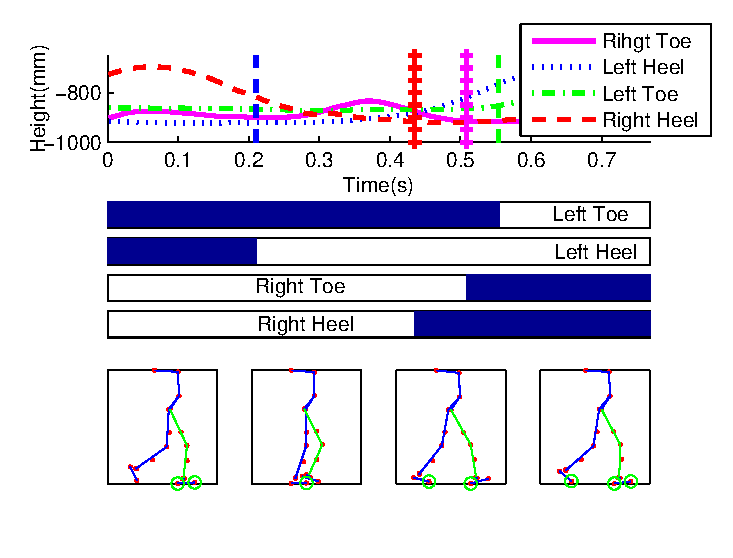
\includegraphics[width=0.8\columnwidth]{domainbreaking}
  \caption[An overview of how the domain breakdown is achieved.]{An overview of
    how the domain breakdown is achieved.
    %
    The top row illustrates the height of the toe and heel of each leg over one
    step along with the lifting and strike time for each constraint (illustrated
    with vertical lines).
    %
    The middle row illustrates which constraints are active based upon the
    fitting.
    %
    The bottom row is the resulting domain breakdown where enforced constraints
    are drawn in green circles.}
  \label{fig:domainbreakdown}
\end{figure}
%
Note: if the data constitute multiple steps, there will be more than one
possible value for $p$;
%
in this case, the proper value of $p$ is the smallest of these values as this
represents one step.
%
The matrix that is premultiplied by $d[n]$ serves the purpose of reordering the
right leg and left leg.
%
If this $p$ can be found, periodic walking over the course of two steps has been
discovered in the data with the behavior of the left leg mirroring the behavior
of the right leg.
%
In this case, one constructs a directed cycle with $p$ domains (as in
\eqref{eq:directedcyclep}) and this is the graph $\Gamma$.
%
The corresponding domain breakdown $\B$ is given by $\B(v_{n}) = d[n]$ for $n
\in \{1, \ldots, p\}$.
%
The application of this procedure to a single subject can be seen in
\figref{fig:domainbreakdown}.


\subsection{Results}

The outlined process is performed on the set of contact points $\C =  \{\clh,
\clt, \crh , \crt\}$ for the nine test subjects that performed the walking
experiment.
%
The end result showed that each subject had the same, {\em universal}, domain
breakdown; this can be seen in \figref{fig:domaingraph}.
%
In the context of this work, a single subject was chosen for study based upon
the completeness of the sensor data, which, in this case, was Subject 4; the
domain breakdown and the time spent in each domain for the subject can be seen
in \figref{fred}.
%
It is important to note that the results are consistent with those found in the biomechanics
literature.
%
Specifically, performing the breakdown process on data from the literature
\cite{Winter2009} resulted in the same domain breakdown.
%
Additionally, the amount of time spent having single and double support are
similar to previous studies \cite{Ackermann2007}.

\begin{figure}[t]
  \centering
  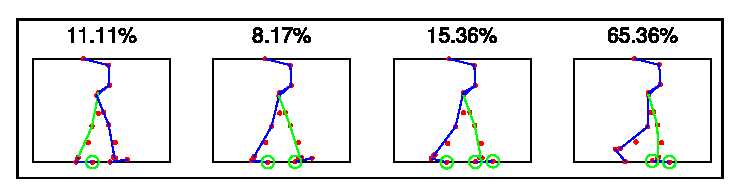
\includegraphics[width=1.0\columnwidth]{test_subject_4}
  \caption{The domain breakdown for Subject 4 together with the amount of
    time spent in each domain.
    %
    Each illustration is a snapshot of the subject's configuration at the
    beginning of the domain together with the contact points enforced.}
  \label{fred}
\end{figure}


\section{Human-Inspired Controller Design}

The goal of this section is to find functions that are ``canonical'' to human
walking, i.e., outputs on the configuration of the human, such as the angle of
the knee, that seem to be intrinsic to walking.
%
These functions will be used in the design of control laws, for a bipedal robot
with anthropomorphic measurements, using the standard method of input/output
linearization \cite{Sastry1999}.
%
This control design strategy results in anthropomorphic walking behavior.


\subsection{``Canonical'' Walking Functions} \label{sec:functions}

Rather than just using trajectories from the human data, functions are sought
which have both ``simple'' representations (much like in the case of heel and
toe height discussed in \secref{sec:domainbreakdown}) and appear to be intrinsic
to human walking.
%
From the perspective of control, these functions must not conflict with the
constraints of the system on each domain resulting from the enforced contact
points as dictated by the domain breakdown.
%
That is, the system must not be overconstrained.

Data are considered from Subject 4 as they contain the least noise; these data
are obtained through the process outlined in \secref{sec:domainbreakdown}.
%
A variety of functions are inspected---these represent different fundamental
behaviors of human walking, e.g., the movement of the torso or of the legs.
%
Examination of the human data, reveals that functions describing the behavior of
the torso, the hip, the non-stance leg slope (the slope of the line connecting
the non-stance ankle to the hip), the knee angles, and the heel and toe heights
seem to encode the most fundamental behaviors related to walking, as dictated by
the correlation between the data and the fitted functions.
%
The human behavior of these different functions throughout the course of the
walking gait can be seen in \figref{fig:constraints-fitting}, with the data
beginning at the start of domain $ts$.

\begin{figure}[t!]
  \centering
  \subfloat[Angular constraints]{
    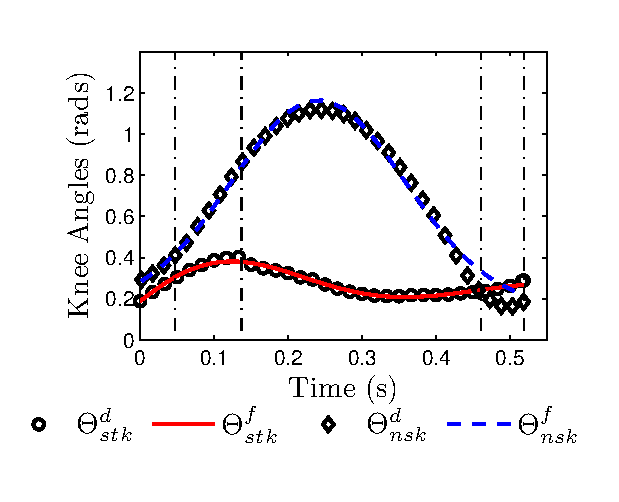
\includegraphics[width=0.48\textwidth]{constraints_angles}
    \label{fig:constraints-knees}
  }
  \subfloat[Slope constraints]{
   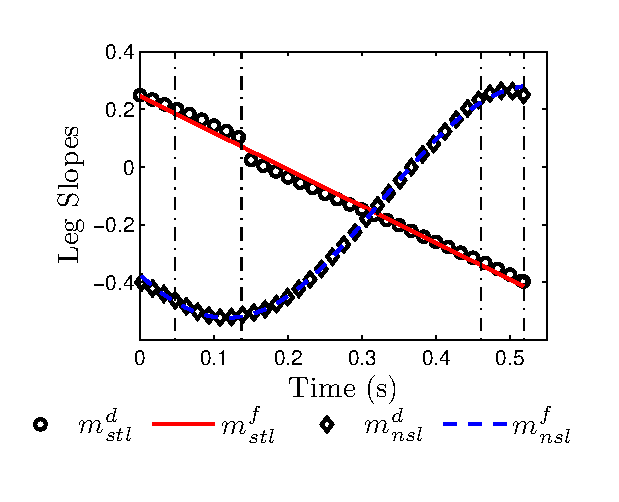
\includegraphics[width=0.48\textwidth]{constraints_slopes}
    \label{fig:constraints-legs}
  }\\
  \subfloat[Height constraints]{
    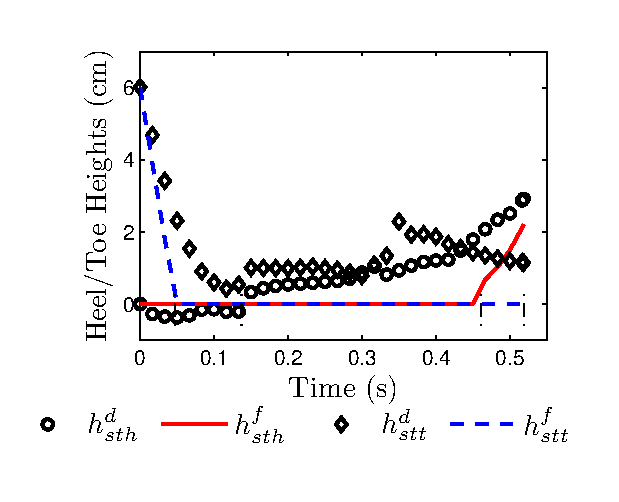
\includegraphics[width=0.48\textwidth]{constraints_heights}
    \label{fig:constraints-heights}
  }
  \caption{Human data over the course of one step with one leg and the
    ``canonical'' functions that are fitted to these data.
    %
    $d$ superscripts represent the data and $f$ superscripts represent the fits.
    %
    The plots start at the beginning of the domain {\DA}, with vertical lines
    indicating when transitions between domains occur.
    %
    The specific variables that are plotted can be seen in
    \figref{fig:robotconstraints}.}
  \label{fig:constraints-fitting}
\end{figure}

Before further detail is given, a remark on the choice of constraints is in
order:
%
\begin{remark} \label{rmk:actuation}
  When choosing which functions to track, it is important to consider which
  joints will have actuation and which actuators will do most of the work
  necessary to track a given constraint.
  %
  An example of a poor choice of constraints would be the stance knee, the
  stance leg slope, and the stance hip position.
  %
  The reason this is a poor choice is as follows:
  %
  to track these three constraints, only two degrees of actuation will do most
  of the work---the stance ankle and the stance knee.
  %
  Thus, the dynamics of the system will be ill-behaved.
  %
  Indeed, if one tries to track three constraints on a two-link pendulum, the
  result will be an overconstrained system {\em unless} two of the constraints
  match up perfectly---in other words, two {\em independent} constraints are
  being tracked.
  %
  This same argument extends to the specified robot, which is a multi-link
  kinematic chain.
  %
  Examples of reasonable output choices can be found in \cite{Sinnet2014}.
\end{remark}


\subsubsection{Knee}

Inspecting the behavior of the human knee over the course of the gait (see
\figref{fig:constraints-knees}) reveals that the angle of the human knee appears
to follow a Gaussian when it is swinging (the non-stance leg) and a second order
system response (i.e., the step response of a spring damper system) when the
weight of the person is on the leg (i.e., when the leg is the stance leg).
%
With this in mind, the following functions are fit to the human data for the
knee angles of the stance and non-stance legs:
%
\begin{align*}
  y_{d,\cnsk}(t) &= A_{5,1} \, \exp\left(\frac{-(t-A_{5,2})^2}{2
      (A_{5,3})^2}\right) + A_{5,4},\\
  y_{d,\cstk}(t) &= -A_{2,1} \, \frac{\cos(A_{2,2}\,t)-A_{2,3}
    \sin(A_{2,2}\,t)}{\exp(A_{2,4} \, t)} + A_{2,5}. 
\end{align*}
%

An intuitive explanation of this is as follows:
%
when the leg is in ``stance'' mode, the human knee acts like a spring-damper
system responding to the impulse of the human as he or she puts his or her body
weight on the stance leg---that is, the human tries to prevent the leg from
collapsing by stiffening it, resulting in a spring-damper effect.
%
When the human leg is in ``non-stance'' mode, the weight of the human is
primarily not on it, so the knee is free to swing---there is no reason to keep
the leg stiff.


\subsubsection{Leg}

In the data for the slope of the non-stance leg as seen in
\figref{fig:constraints-legs}---here, leg is defined as the straight line
connecting the ankle to the hip---the slope appears to follow a sinusoid; thus
the following function is fit:
%
\begin{align*}
  y_{d,nslm}(t) &= A_{6,1} \, \sin(A_{6,2} \, t + A_{6,3}) + A_{6,4}.
\end{align*}
%
Intuitively, this just means that the non-stance leg swings freely much like the
non-stance knee.
%
Note that while it is possible to choose the slope of the stance leg as a
constraint to track---indeed, a simple function can be fitted to the slope of
the stance leg---the forward velocity of the hip is instead chosen.
%
In terms of time-control this will not make much of a difference, but the reader
will see that, when the control is migrated to pure feedback, tracking the hip
velocity will allow for direct control over walking speed.


\subsubsection{Hip}

The behavior of the hip is quite simple.
%
Examination of the data reveals that the hip moves forward monotically in time
at an approximately constant rate.
%
However, instead of tracking the position of the hip, the velocity of the hip is
instead tracked, thus motivating the following function:
%
\begin{align*}
  y_{d,hv} = A_{3,1}.
\end{align*}
%
The reason for tracking the velocity instead of the position is related to the
method used to impose feedback control on the system and requires some
explanation; however, due to the level of detail, this discussion will be
deferred until later.
%
It is of interest, however, to note that, as mentioned previously, tracking hip
velocity allows for direct control over the walking speed of the robot.


\subsubsection{Torso}

The data show that a human tends to keep his or her torso upright throughout his
or her walking gait.
%
Specifically, the data indicates that the absolute angle of the torso with
respect to the world frame closely follows a sine wave, but the amplitude is
small, so it is approximated with a constant:
%
\begin{align*}
  y_{d,T\angle} &= A_{4,1}.
\end{align*}
%
Note that, the choice of tracking a constant results in a poor correlation
between the function and data; however, one can argue that the tiny amount of
motion from the torso has very little effect on the overall gait.


\subsubsection{Ankle}

When the non-stance leg is swinging, to prevent the non-stance ankle from
rotating freely, the behavior of the ankle angle is approximated by a constant:
%
\begin{align*}
  y_{d,nsa\angle} &= A_{8,1}.
\end{align*}
%
One can justify this choice by claiming that the motion of the ankle has only a
marginal effect on the overall gait provided that ground clearance is not an
issue.
%
As in the case of the torso, the correlation between this fit and the data will
not be good but, again, this does not have a large effect on the gait.


\subsubsection{Foot}

Finally, the behaviors of the heel and toe are found to be significantly more
complicated than the previously discussed behaviors, as can be seen in
\figref{fig:constraints-heights}.
%
Although the actual functions describing these heights are quite simple (see
\figref{fig:heeltoefit}), it is generally not effective to follow these
functions---see \rmkref{rmk:dimconst}.
%
Since the foot is constrained during certain phases of the gait, it would not
make sense to track the constrained points during these phases.
%
Therefore, the behavior of the feet is segmented based on the domain breakdown
of the human gait.
%
In particular, the transition from domain {\DA} to domain {\DB} occurs when the
stance toe strikes the ground, and, in fact, it is found that the height of the
toe approximately follows a constant as it approaches the ground in domain
{\DA}.
%
In order to satisfy this local objective, an attempt is made to track the height
of the toe using the following function:
%
\begin{align*}
  y_{d,\cstth}(t) = A_{7,1} \, t + A_{7,2}.
\end{align*}
%
After domain {\DA}, the toe is fixed to the ground and thus, is no longer
tracked.
%
In a similar light, when domain {\DC} is reached, the goal is to effect heel
lift.
%
As such, analysis of the data reveals that non-stance heel begins to lift
approximately according to a Gaussian, thus motivating the following function:
%
\begin{align*}
  y_{d,\csthh}(t) &= A_{1,1} \, \exp\left(\frac{-(t-A_{1,2})^2}{2 (A_{1,3})^2}\right) + A_{1,4}.
\end{align*}

\begin{remark} \label{rmk:dimconst}
  Certain constraint functions represent dimensionalized constraints, e.g., heel
  height, whereas other functions discussed, e.g., angles and slopes, represent
  nondimensionalized constraints.
  %
  In general it is not effective to follow dimensionalized constraints as they
  represent constraints on specific points of the system and thus have the
  potential to introduce extreme restrictions on the configuration space of the
  entire system.
  %
  This should be thought of in terms of the inverse kinematics problem:
  %
  consider an end-effector and solve for the range of possible configurations on
  the angles leading up to that point.
  %
  Thus, dimensionalized constraints are not robust with respect to length
  parameters.
  %
  Additionally, these dimensionalized constraints can conflict with other
  holonomic constraints being tracked.
  %
  Recall that the intent is to track the height of the stance toe;
  %
  in this case, the issue of configuration restriction is minimal:
  %
  only the heel is pinned to the ground so tracking the toe's height is
  equivalent to tracking the angle or slope of the foot.
\end{remark}

\begin{figure}[t!]
  \centering
  \subfloat[Robot configuration]{
    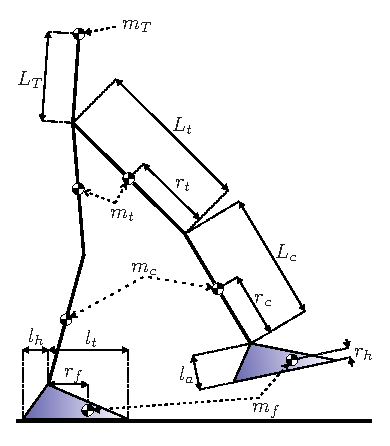
\includegraphics[width=.4\columnwidth]{robot_config}
    \label{fig:roboconf}
  }
  \hspace{.2cm}
  \subfloat[Tracking outputs]{
    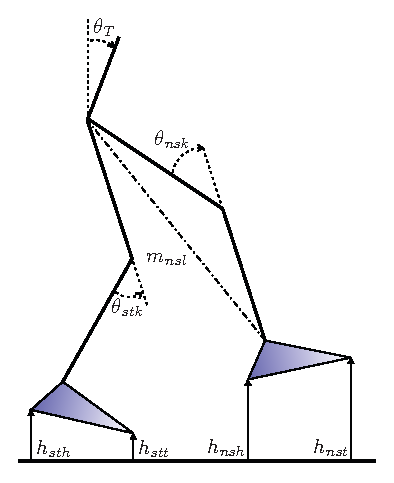
\includegraphics[width=.4\columnwidth]{robot_const}
    \label{fig:trackingoutputs}
  }
  \caption[Kinematic and dynamic model of the 2D bipedal robot.]{Kinematic and
    dynamic model of the 2D bipedal robot:
    % 
    (a) The general configuration of the 2D bipedal robot with knees and feet;
    % 
    (b) The different configuration-based outputs considered in the fitting of
    the ``canonical'' functions.}
  \label{fig:robotconstraints}
\end{figure}


\subsubsection{Fitting}

The paramaters of the ``canonical'' functions can be found by minimizing the
error between the human data and the corresponding functions.
%
Formally, given a function choice $y_d(t, A)$, with $A \in \R^{n_{d}}$ the $n_d$
parameters, and the corresponding data function $x_{d}[k]$ with indexed time
$\tau_{d}[k]$ for data index $k \in \{1, \ldots, K\}$ (for $K$ data points), a
solution is sought for the optimization problem:
%
\begin{align}
  \label{eq:fitsolve}
  \min_{A \in \R^{n_{d}}} \sum_{k=1}^{K} (y_{d}(\tau_{d}[k], A) - x_{d}[k])^2.
\end{align}
%
The fits that result from solving \eqref{eq:fitsolve} are shown in
\figref{fig:constraints-fitting}.
%
The correlation coefficient for the fits of each of the respective functions can
be found in \tabref{tab:fitcor}.
%
In all cases (with the exception of the torso and ankle), the fits are very
good.
%
One final note of import:
%
in order to achieve walking in simulation, some parameters had to be tweaked by
hand;
%
the parameters generated as well as the tweaked parameters can be found in
\tabref{tab:funcparam}.

\begin{table*}[t!]
  %\HRule
  \centering
  \caption[Correlations of fitted functions and usage on each
  domain.]{Correlations of fitted functions and usage on each domain.
    %
    Note that many fits have extremely high correlations.
    %
    For the four right columns, a $\bullet$ indicates the constraint for that
    row is tracked on the corresponding domain.
  }
  \begin{tabular}{| c | l | c || c | c | c | c |}
    \hline
        {\bf Eq.} & {\bf Constraint} & $r$ & $\DA$ & $\DB$ & $\DC$ & $\DD$\\
        \hline
        $y_{d,sthh}$ & Stance heel height & 0.73671 & & & & $\bullet$ \\
        \hline
        $y_{d,stk\angle}$ & Stance knee angle & 0.99213 & $\bullet$ & $\bullet$
        & $\bullet$ & $\bullet$ \\
        \hline
        $y_{d,hv}$ & Hip forward velocity  & * & $\bullet$ & $\bullet$ &
        $\bullet$ & $\bullet$ \\
        \hline
        $y_{d,T\angle}$ & Torso absolute angle & * & $\bullet$ & $\bullet$ &
        $\bullet$ & $\bullet$ \\
        \hline
        $y_{d,nsk\angle}$ & Non-stance knee angle & 0.99301 & $\bullet$ &
        $\bullet$ & $\bullet$ & $\bullet$ \\
        \hline
        $y_{d,nslm}$ & Non-stance leg slope & 0.99971 & & & $\bullet$ & \\
        \hline
        $y_{d,stth}$ & Stance toe height & 0.99971 & $\bullet$ & & &\\
        \hline
        $y_{d,nsa\angle}$ & Non-stance ankle angle & * & & & $\bullet$ &
        $\bullet$\\
        \hline
  \end{tabular}
  \label{tab:fitcor}
\end{table*}

\begin{table}[t!]
  % \HRule
  \caption[Human function parameters.]{Human function parameters.
    %
    Asterisks (*) denote no additional parameters.}
  \centering
  \begin{align*}
    A = \left[\begin{array}{c c c c c}
        % sthh
        0.2039 & 0.7540 & 0.1109 & 0.0000 & *\\
        % stka
        0.0710 & 13.3920 & 2.6671 & 3.7440 & 0.1881\\
        % hv
        1.1771 & * & * & * & *\\
        % Ta
        0.0595 & * & * & * & *\\
        % nska
        1.1500 & 0.2480 & 0.1170 &0.1669 & *\\
        % nslm
        0.4035 & 7.5204 & -2.4442 & -0.1202 & *\\
        % stth
        -0.1638 & 0.0078 & * & * & *\\
        % nsaa
        -0.0800 & * & * & * & *        
      \end{array}\right]
  \end{align*}
  \label{tab:funcparam}
\end{table}



\subsection{Robotic Hybrid Model \& Controllers}

Consider the robotic walker shown in \figref{fig:robotconstraints}.
%
The goal is to use the human-inspired domain breakdown and ``canonical'' walking
functions to design controllers for this robot.


\subsubsection{Robotic Model}

It was shown in \secref{sec:complex-models} that, given a collection of contact
points and a domain breakdown (defined on a cycle graph), one can explicitly
construct a hybrid control system.
%
In particular, using the procedure discussed, a domain breakdown $\B$ is
obtained, which is associated to human walking (see
\exmpref{ex:domainbreakdown}) defined on the cycle $\Gamma_u = (V, \, E)$ (given
in \exmpref{universalgraph}).
%
As a result of the construction in \secref{sec:complex-models}, one obtains a
hybrid control system describing this robot:
%
\begin{align}
  \label{eq:hcstime}
  \HCS = (\Gamma, \D, \U, \Guard, \Delta, \FG).
\end{align}
%
\begin{figure}[t!]
  \centering
  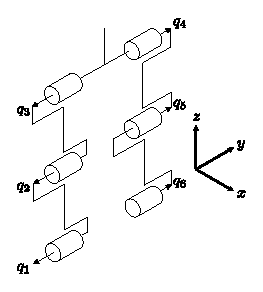
\includegraphics[width=.45\columnwidth]{robot_angles}
  \caption[The shape coordinates for the biped labeled $q_i$.]{The shape
    coordinates for the biped labeled $q_i$.
    %
    The corresponding arrows represent twists. The $x$-axis is coming out of the
    page.
    %
    The hip width is zero and is shown for illustration purposes only.
    %
    The axes shown represents the body-fixed frame which has orientation about
    the $y$-axis given by $\phi_b$.}
  \label{fig:shapecoords}
\end{figure}
%
As discussed previously, attach a reference frame $\Rb$ to the hip. Let $\phi_b$
be the orientation of $\Rb$ (with respect to the $y$-axis for a two-dimensional
model) and let $p_b^x, p_b^z$ be the Cartesian position of $\Rb$.
%
The shape coordinates $\qs$ for the biped are chosen to be the relative angles
between any two successive links starting at the stance foot as shown in
\figref{fig:shapecoords}.
%
Combining $\phi_b$, $p_b^x$, $p_b^z$, and $\qs$ gives the configuration space
for the biped.
%
The only unknowns for the model are the physical parameters of the system;
%
these are obtained from the anthropometric data for Subject 4, given in
\tabref{tab:measurements}.
%
In particular, the lengths are given and the mass of each point mass in the
robot (as seen in \figref{fig:robotconstraints}) is estimated from the overall
mass of the person using a standard mass distribution of a human from the
literature \cite{Winter2009}.


\subsubsection{Controller Design}

The goal now is to design a controller to track the desired functions given in
\secref{sec:functions}.
%
Before discussing which of these functions are tracked on each domain, a
description technique used to track the desired functions, input/output
linearization \cite[Ch.~9]{Sastry1999}, is given. % Sastry, pp. 407

Consider a control system of the form $(\xfv, \, \xgv)$, $\vinV$ as given in
\defref{def:hcs} for an arbitrary domain in the domain breakdown.
%
Let $y^{a}_{v}\argsq$ represent the vector of ``actual'' outputs on the system
(e.g., the height of the stance heel)---these can be found by computation of
forward kinematics \cite{Murray1994}.
%
Let $y^{d}_{v}\argt$ represent the vector of ``desired'' output functions to be
tracked, which consists of combinations of the human-based ``canonical''
constraint functions.
%
Let $n = \dim(Q)$ and let $m$ be the number of constraint functions being
tracked on a given domain.
%
Motivated by the desire to drive $y^{a}_{v}(\q\argt) \to y^{d}_{v}\argt$ as $t
\to \infty$, a definition is given for the following virtual output vector:
%
\begin{align}
  \label{eq:virtout}
  y_v(\q, t) = y^a_v\argsq - y^d_v\argt.
\end{align}
As the functions tracked consists of both positions and velocities, the system
has mixed relative degree.
%
That is, the output corresponding to velocity will have relative degree one
whereas the outputs corresponding to positions will each have relative degree
two.
%
Reorder the outputs as follows:
\begin{align}
  \label{eq:vouts}
  y_v(\q, \dq, t) = (y_{v,1}(\q, \dq, t), y_{v,2}(\q, t))
\end{align}
with $y_{v,1}$ a vector containing the relative-degree-one outputs and $y_{v,2}$
a vector containing the relative-degree-two outputs.
%
(In this thesis, $y_{v,1}$ is a scalar.)
%
A control law which drives \eqref{eq:vouts} to zero is
\begin{align*}
  \lefteqn{u(\q, \dq, t) = }\\
  &&-\mathcal{A}_{v}^{-1}(\q, \dq, t)
  \left(\left[\!\!\begin{array}{c}
      0\\
      L_{\xfv} L_{\xfv} y_{v,2}(\q, t)
    \end{array}\!\!\right]
  + \left[\!\!\begin{array}{c}
      L_{\xfv} y_{v,1}(\q, \dq, t)\\
      2 \varepsilon L_{\xfv} y_{v,2}(\q, t)
    \end{array}\!\!\right] +
  \left[\!\!\begin{array}{c}
      \varepsilon y_{v,1}(\q, \dq, t)\\
      \varepsilon^2 y_{v,2}(\q, t)
    \end{array}\!\!\right]\right),
\end{align*}
with $\mathcal{A}_{v}(\q, \dq, t)$ the decoupling matrix given by
\begin{align*}
  \mathcal{A}_{v}(\q, \dq, t) =
  \left[\begin{array}{c}
      L_{\xgv} y_{v,1} (\q, \dq, t)\\
      L_{\xgv} L_{\xfv} y_{v,2}(\q, t)
    \end{array}\right],
\end{align*}
where, again, $(\xfv, \, \xgv)$ is given in \defref{def:hcs}.
%
In the above,
\begin{align*}
  L_{\xfv} y(\q, \dq, t) = \pd{y(\q, \dq, t)}{(\q, \dq, t)} \cdot
  \xfv(\q, \dq, t)
\end{align*}
represents the Lie derivative with $\q, \dq, t$ representing independent
variables.
%the control field $g_v(q)$ is given by
%\begin{align}
%    g_v(q) = \left[\begin{array}{c}
%        \mathbf{0}_{n \times m}\\
%        D^{-1}(q) B(q)
%    \end{array}\right]
%\end{align}
%with $B(q)$ a torque distribution matrix specific to each domain. These are
%omitted but can be found online at \cite{SUP_online}.
Applying the given control law yields the non-autonomous closed-loop dynamical
system
\begin{align}
  \label{eq:clsys}
  \xf_\mathit{cl,v}(\q, \dq, t) = \xfv(\q, \dq) + \xgv\argsq \, \uu(\q, \dq, t).
\end{align}
%The corresponding hybrid system is then
%\begin{align}
%    \HS = (\D, S, R, F)
%\end{align}

Completion of the controller construction requires the specification of the
vectors $y^{a}_{v}$ and $y^{d}_{v}$ for $\vinV$ which are specific to each
of the four domains in \figref{fig:domaingraph}.
%
As mentioned previously, the vector $y^a_v$ consists of the robotic constraints
pictured in \figref{fig:robotconstraints}, which are computed directly from the
kinematics of the robot.
%
Therefore, the only decision remaining is which of the ``canonical'' human
functions to track on each domain.
%
The specific choice of functions is shown in \tabref{tab:fitcor} where black
dots indicate which functions are tracked on which domains.
%
The choice of functions is based on the discussion in \secref{sec:functions}
coupled with choosing collections of functions that do not conflict with the
holonomic constraints imposed on the system as a result of ground contact (see
Remarks \ref{rmk:actuation} and \ref{rmk:dimconst}).
%
Applying these collections of controllers to the hybrid control system
\eqref{eq:hcstime} yields the non-autonomous hybrid system:
%
\begin{align}
  \label{eq:hstime}
  \HS_{t} = (\Gamma, \, \D, \, \Guard, \, \Delta, \, \F).
\end{align}

\begin{remark}
  One final point worthy of mention is transitioning from domains with no
  impact, i.e., contact point becomes unconstrained.
  %
  Looking at equations, \eqref{eq:controlsystem} and \eqref{eq:wrench}, it is
  apparent that one can achieve lift by simply solving for a value of $\uu$
  which will cause the heel to lift.
  %
  Such a value would be outside the domain as defined in \eqref{eq:domain};
  %
  specifically, this value of $\uu$ will violate \eqref{eq:constnu}.
  %
  Provided that \eqref{eq:constnu} is satisfied during the a given phase, it
  becomes a control decision when to lift the heel or toe.
  %
  A criterion is chosen and then appropriate control is applied to
  instantaneously achieve heel or toe lift.
  %
  In the domain that follows, the control laws implicit in \eqref{eq:clsys} will
  be responsible for causing the toe or heel to continue to lift.
\end{remark}


\subsection{Simulation of Time-Based Feedback Controller} \label{sec:timesim}

This subsection presents the results of a simulation of the bipedal robot
modeled by \eqref{eq:hstime}.
%
The parameters used for the human functions are given in \tabref{tab:funcparam}.
%
It is important to note that, in order to achieve walking, it was necessary to
tweak the parameters;
%
specifically, this amounted to the multiplication of the row corresponding to
the non-stance leg slope (row six) by $1.25$.
%
Videos of the walking can be found online.%
%
\footnote{\url{http://www.rwsinnet.com/phdthesis/}\label{fn:rwsinnet}}\xspace
%
It is found through simulation that the biped has stable walking.
%
This is checked by finding a fixed point on the orbit and verifying its
stability using the \Poincare{} map technique \cite{Parker1989}.
%
Using the model parameters found online\fnref{fn:rwsinnet} and the
input/output linearization control gain $\varepsilon = 15$, the system is
simulated and the following fixed point is found:
%
\begin{align}
  q_{s,t}^{*} =
  \left(\!\!\!\!\begin{array}{c c c c c c}
    -.460 & \hphantom{-}.246 & \hphantom{-}.272 & -.441 & \hphantom{-0}.323 &
    \hphantom{-}.162
  \end{array}\!\!\right)\\
  {\dot q}_{s,t}^{*} =
  \left(\!\!\!\!\begin{array}{c c c c c c}
    -.951 & \hphantom{-}.452 & \hphantom{-}.518 & -.309 & -2.660 & -.509
  \end{array}\!\!\right)
\end{align}
which is on the guard of domain $\DC$.
%
This verifies that there exists a walking gait.
%
Note that only the shape coordinates are given for the fixed point as the other
coordinates will be completely determined by the condition that the biped is on
the guard;
%
that is, the constraints that exist on the system, e.g., the stance toe is on
the ground, are enough to uniquely determine the rest of the variables,
$\phi_b$, $p_x$, and $p_z$.

In the context of bipedal walking, a stable limit cycle or an exponentially
stable periodic orbit implies stable walking.
%
It is, therefore, desirable to show that the system has a stable limit cycle.
%
This is achieved by examining the Jacobian of the \Poincare{} map linearized
about the fixed point $(\qst, \dqst)$ \cite{Parker1989}.
%
This \Poincare{} map will be stable if all the eigenvalues of the Jacobian have
magnitude below unity.
%
Then, stability of the \Poincare{} map implies stability of the system.
%
The Jacobian matrix can be approximated by perturbing along the guard about the
fixed point with respect to the coordinates $\q$ and $\dq$.
%
A numerical approximation yields eigenvalues of the following magnitudes:
%
\begin{align}
  \label{eq:time-eigs}
  |\lambda_{t}| \in \{0.2640, \, 0.2492, \, 0.0337, \, 0.0337, \, 0.0011, \,
  \ldots\},
\end{align}
where, for the sake of space, only the five eigenvalues with the largest
magnitudes are included.
%
At this point in the discussion, a remark about zero eigenvalues is appropriate:

\begin{remark}
  When considering a \Poincare{} section $\Guard$ which is a guard of a hybrid
  system with constraints, some of the eigenvalues will be zero.
  %
  This is a result of the difference in the dimension of the Jacobian and the
  dimension of the guard which is a transverse hyperplane of the continuous
  trajectory.
  %
  Specifically, consider the guard used here as $\Guard$.
  %
  In this  case, the guard restricts the previously nine-dimensional position
  space such that the state of the system, throwing out cyclic variables such as
  $x$-position, can be determined completely using only six position variables.
  %
  This results in a number of zero eigenvalues, in this case, three relating to
  position and three for the corresponding velocities.
  %
  More on this topic can be found in the literature \cite{Wendel2010}.
\end{remark}

The eigenvalues in \eqref{eq:time-eigs} have magnitude below unity, and thus,
the system has a locally exponentially stable periodic orbit.
%
The phase portraits are shown in \figref{fig:pp-t}.
%
These phase portraits are closed---in other words, they contain a closed
periodic orbit.
%
\begin{figure*}[t!]
  \centering
  \subfloat[Body frame angle]{
    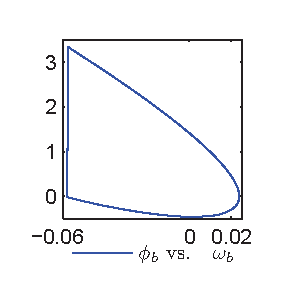
\includegraphics[width=0.24\textwidth]{pp-time-1-s}
    \label{fig:pp-t-ref}
  }
  \subfloat[Ankle angles]{
    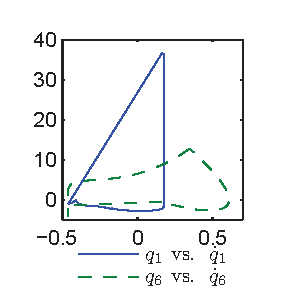
\includegraphics[width=0.24\textwidth]{pp-time-2-s}
    \label{fig:pp-t-ankle}
  }
  \subfloat[Knee angles]{
    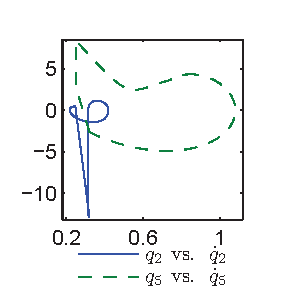
\includegraphics[width=0.24\textwidth]{pp-time-3-s}
    \label{fig:pp-t-knee}
  }
  \subfloat[Hip angles]{
    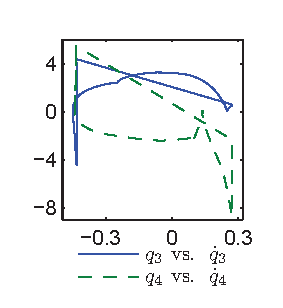
\includegraphics[width=0.24\textwidth]{pp-time-4-s}
    \label{fig:pp-t-hip}
  }
  \caption{Phase portraits of simulation of time-based system $\HS_t$.}
  \label{fig:pp-t}
\end{figure*}
%
\begin{figure}[t!]
  \centering
  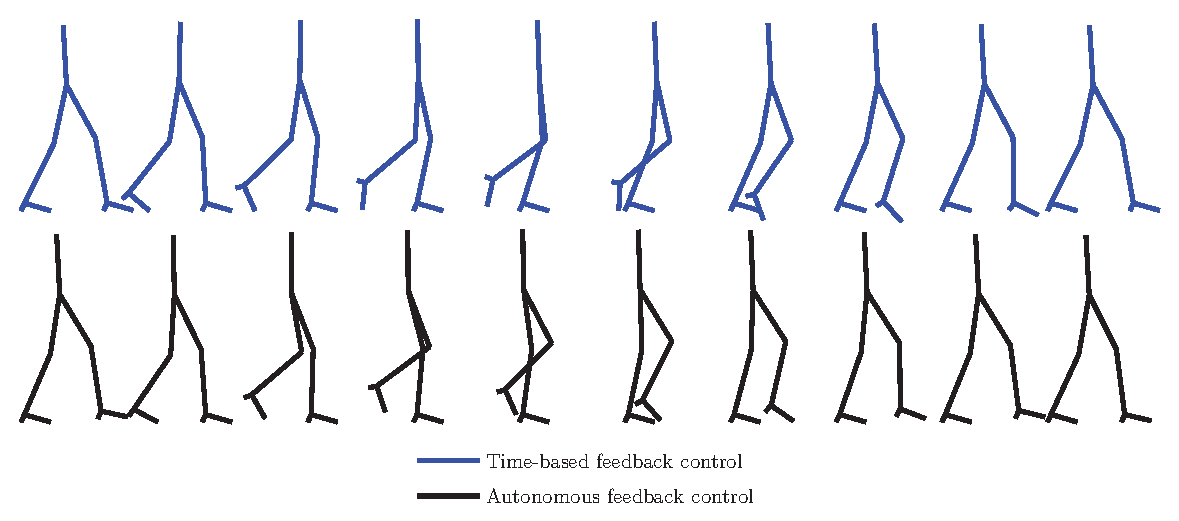
\includegraphics[width=1.0\textwidth]{hic_gait_tiles}
  \caption[Comparison of simulated walking gaits.]{Comparison of simulated
    walking gaits. Time-based feedback control and autonomous feedback
    control.}
  \label{fig:gaittiles}
\end{figure}
%
Snapshots of the walking gait are shown in \figref{fig:gaittiles}.
%
These simulation results imply that, through a choice of functions intrinsic to
human walking, humanlike walking was indeed obtained for on an anthropomorphic
biped.
%
The humanlike nature of the simulated gait can best be seen in a video of the
walking available online.\fnref{fn:rwsinnet}


\section{Autonomous Feedback Controller Design}

In general, autonomous control is preferred over non-autonomous, time-based
control as autonomous controllers tend to be more robust.
%
In this section, a method is given which shows how to remove the time-dependence
from the ``canonical'' functions described in the previous section.
%
A common trick in the literature \cite{Westervelt2007} for converting time-based
trajectories into state-based trajectories is to parameterize time by a
state-dependent function;
%
this results in an autonomous feedback control strategy.

\begin{figure}[t]
  \centering
  \subfloat[Comparison of hip movement] {
    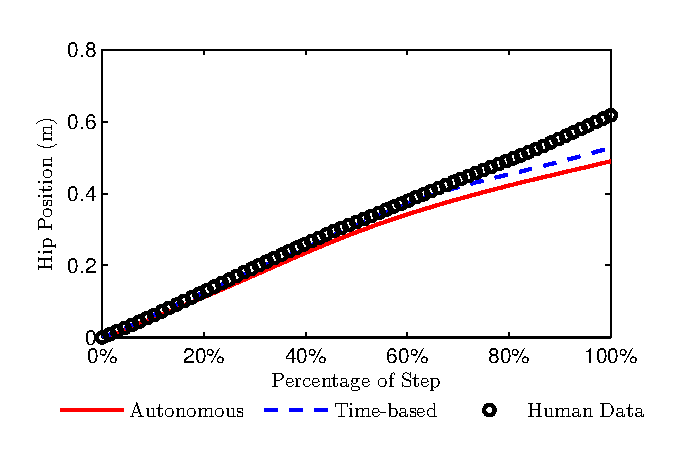
\includegraphics[width=.48\textwidth]{hip_pos}
    \label{fig:hip-pos}
  }
  \subfloat[Angular motion of torso] {
    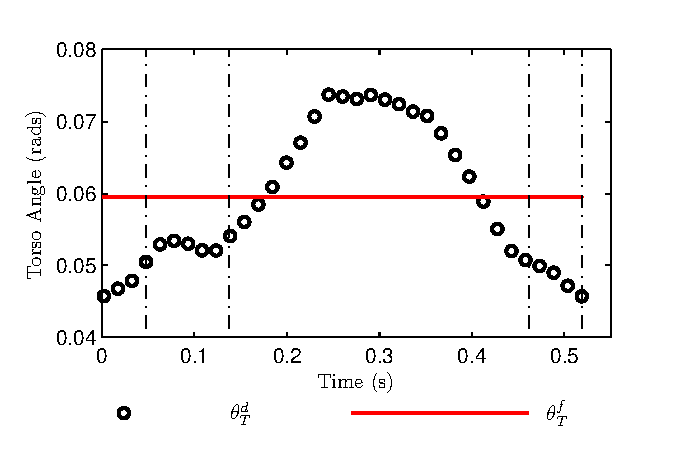
\includegraphics[width=.48\textwidth]{torso_angle}
    \label{fig:torso-angle}
  }
  \caption{Trajectories for the hip (a) and torso (b).}
  \label{fig:torso-hip}
\end{figure}


\subsection{State-Based Trajectory Parameterization}

Recall that the functions discussed in the previous section are directly
dependent on time, i.e., they can be written $y_{\vo}^{d}\argt$.
%
Furthermore, these functions are all defined on some interval $[t^{-} = 0, t^{+}
= P] = \mathcal{I} \subset \R_{0}^{+}$ with $P$ the period of the gait (that is,
one step with one leg);
%
in other words, a given tracking function can be written as a map $y_{\vo}^{d} :
\mathcal{I} \to \R$.
%
Autonomous state feedback can be achieved by simply choosing a state-based
parameterization $\varsigma : \Q \to \mathcal{I}$ and substituting for time,
i.e., $y_{\vo}^{d}(\varsigma\argsq)$.

When choosing a parameterization, $\varsigma\argsq$, it is important to consider
its role in the system.
%
Since $\varsigma\argsq$ is a parameterization for time $t$, the relationship
between $\varsigma\argsq$ and $t$ should be as linear as possible.
%
Examination of the human hip data, as shown in \figref{fig:hip-pos}, reveals
that the hip velocity $v_{\mathit{hip}}^{x}$ is constant throughout the gait;
%
as a result, the hip position approximately satisfies
$p_{\mathit{hip}}^{x}(\q\argt) = v_{\mathit{hip}}^x t + p_\mathit{hip}^x(\qm)$,
with $\qm$ the state at the beginning of a step.
%
Here, the assumption can be made, without loss of generality, that time starts
at zero at the beginning of any given step.
%
The linearity of the hip position, $p_{\mathit{hip}}^{x}(\q\argt)$, with respect
to time, makes it a good candidate for time parameterization;
%
substituting $\varsigma\argsq \to t$ and solving for $\varsigma\argsq$ gives the
parameterization
\begin{align}
  \label{eq:prm}
  \varsigma\argsq = \frac{p_{\mathit{hip}}^{x}\argsq -
    p_{\mathit{hip}}^{x}\argsqm}{v_{\mathit{hip}}^{x}}.
\end{align}
%
The parameters $p_{\mathit{hip}}^{x}\argsqm$ and $v_{\mathit{hip}}^{x}$ should be
chosen based on the quantities they represent (i.e., $v_{\mathit{hip}}^{x}$
should be the average velocity of the hip and $p_{\mathit{hip}}^{x}\argsqm$ should
be the $x$-position of the hip at the beginning of a step).
%
In this work, these values were found by examining the simulation of the
time-based controller from the previous section.
%
Specifically, a good choice for $v_{\mathit{hip}}^{x}$ is the parameter for the
hip velocity constraint, $A_{3,1}$ (found in \tabref{tab:funcparam}).
%
Using the parameterization \eqref{eq:prm}, the desired trajectories can be
expressed by substituting the parameterization $\varsigma\argsq$ for time $t$;
%
that is, the desired trajectories will be given by
$y_{\vo}^{d}(\varsigma\argsq)$.


\subsubsection{Control Design Modification}

Implementation of state feedback allows for the removal of time from the virtual
outputs, that is, the control law is no longer time-dependent.
%
Therefore, the virtual output of \eqref{eq:virtout} becomes
\begin{align*}
  y_{\vo}\argsqdq = y_{\vo}^a\argsqdq - y_{\vo}^{d}(\varsigma\argsq)
\end{align*}
with $\varsigma\argsq$ the parameterization given in \eqref{eq:prm}.
%
Following the derivation of the time-based controller, the outputs are grouped
based on relative degree:
%
\begin{align*}
  y_{\vo}\argsqdq = (y_{\vo,1}\argsqdq, y_{\vo,2}\argsq).
\end{align*}
%
The control law which drives $y_{\vo}\argsqdq \to 0$ is then given by
\begin{align*}
  \uu\argsqdq = -\mathcal{A}_{\vo}^{-1}\argsqdq \left(
  \left[ \begin{array}{c}
      0\\
      L_{\xf_{\vo}} L_{\xf_{\vo}} y_{\vo,2}\argsq
    \end{array} \right] +
  \left[ \begin{array}{c}
      L_{\xf_{\vo}} y_{\vo,1}\argsqdq\\
      2 \varepsilon L_{\xf_{\vo}} y_{\vo,2}\argsq
    \end{array} \right] +
  \left[ \begin{array}{c}
      \varepsilon y_{\vo,1}\argsqdq\\
      \varepsilon^2 y_{\vo,2}\argsq
    \end{array} \right]\right),
\end{align*}
with $A_{\vo}(q)$ the decoupling matrix given by
\begin{align}
  \mathcal{A}_{\vo}\argsqdq =
  \left[\begin{array}{c}
      L_{\xg_{\vo}} y_{\vo,1} \argsqdq\\
      L_{\xg_{\vo}} L_{\xf_{\vo}} y_{{\vo},2}\argsq
    \end{array}\right]
\end{align}
and $(\xf_{\vo}, \, \xg_{\vo})$ the control system given in
\eqref{eq:controlsystem}.
%
Application of this control law to the control system yields the closed-loop
system:
%
\begin{align}
  \xf_{cl,\vo} = \xf_{\vo}\argsqdq + \xg_{\vo}\argsq \, \uu\argsqdq.
\end{align}
%
The virtual outputs are chosen to be the same as those in the time-based
controller, specified in \tabref{tab:fitcor}.
%
The end result is an autonomous hybrid system specified by
\begin{align}
  \HS_{a} = (\Gamma, \, \D, \, \Guard, \, \Delta, \, \F_{a}).
\end{align}
with $\F_{a}$ the set of vector fields $\{\xf_{cl,\vo}\}_{\vo \in V}$.


\begin{figure*}[tp!]
  \centering
  \subfloat[Body frame angle]{
    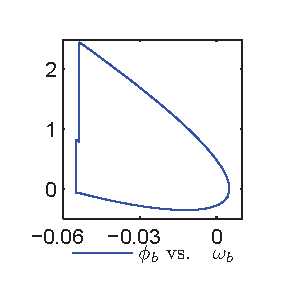
\includegraphics[width=0.24\textwidth]{pp-auto-1-s}
    \label{fig:pp-a-ref}
  }
  \subfloat[Ankle angles]{
    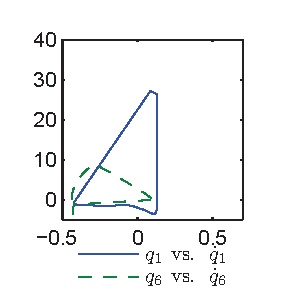
\includegraphics[width=0.24\textwidth]{pp-auto-2-s}
    \label{fig:pp-a-ankles}
  }
  \subfloat[Knee angles]{
    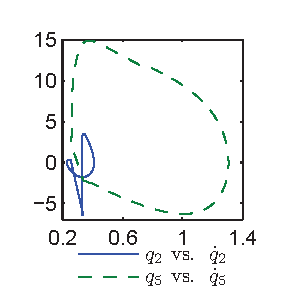
\includegraphics[width=0.24\textwidth]{pp-auto-3-s}
    \label{fig:pp-a-knee}
  }
  \subfloat[Hip angles]{
    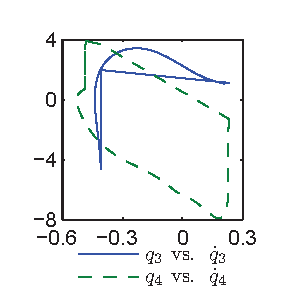
\includegraphics[width=0.24\textwidth]{pp-auto-4-s}
    \label{fig:pp-a-hip}
  }
  \caption{Phase portraits of simulation of autonomous system $\HS_{a}$.}
  \label{fig:pp-a}
\end{figure*} 


\subsection{Simulation of Autonomous Feedback Controller}

The analysis of the stability of the autonomous system is analogous to that
shown in \secref{sec:timesim}.
%
The control gain is again chosen to be $\varepsilon = 15$.
%
The parameters are tweaked, as before, by multiplying row six by $1.25$.
%
This simulation results in the fixed point:
%
\begin{align*}
  \qst_{s,t} &=
  \left(\begin{array}{r r r r r r}
      -\hphantom{1}.404 & .245 & \hphantom{1}.208 & -\hphantom{0}.488 &
      \hphantom{-2}.388 & \hphantom{-}.088
  \end{array}\right)\\
  \dqst_{s,t} &=
  \left(\begin{array}{r r r r r r}
    -1.287 & .282 & 1.078 & \hphantom{-}0.711 & -2.452 & -.076
  \end{array}\right)
\end{align*}
on the guard of domain {\DC}.
%
Only the shape coordinates are shown, as in the analysis of the time-based
feedback controller.
%
The Jacobian matrix of a linearization of the \Poincare{} map about the fixed
point $(\qst_{s}, \dqst_{s})$ yields eigenvalues of the following
magnitudes:
%
\begin{align*}
  |\lambda_{a}| \in \{0.1902, \, 0.0680, \, 0.0680, \, 0.504, \, 0.0058, \,
  \ldots\},
\end{align*}
where, again, only the five eigenvalues with the largest magnitudes are shown.
%
The phase portraits are shown in \figref{fig:pp-a}.
